\documentclass[border=10pt]{standalone}
\usepackage[svgnames]{xcolor}
\usepackage{amsmath}
\usepackage{pgfplots}
\pgfplotsset{compat=newest}
\usepackage[sfdefault]{FiraSans}
\usepackage{FiraMono}
\renewcommand*\familydefault{\sfdefault}
\begin{document}
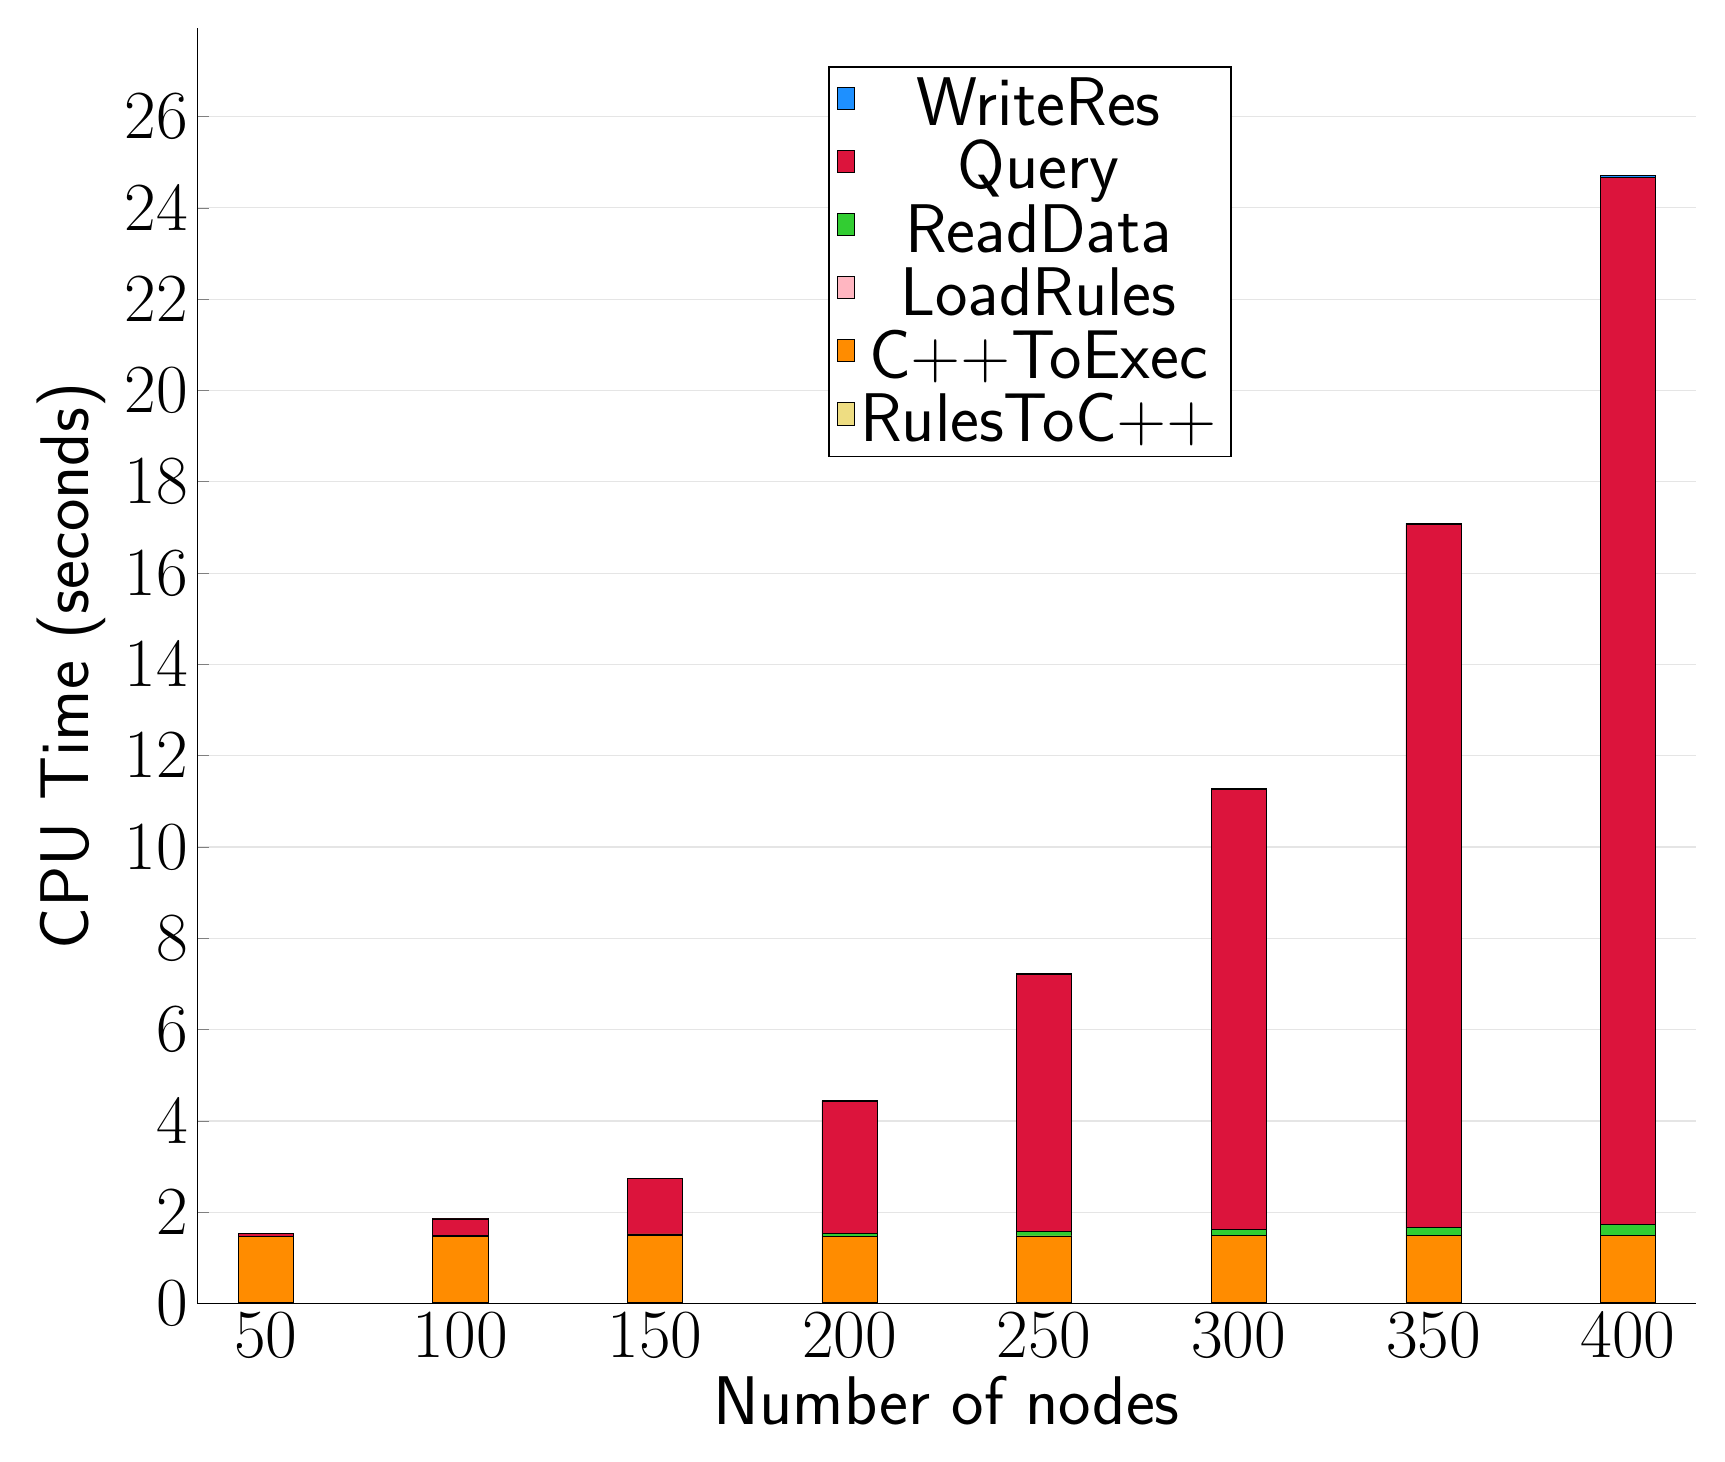
\begin{tikzpicture}
\begin{axis}[
   ybar stacked,
   width=1.7\textwidth,
   bar width=0.7cm,
   ymajorgrids, tick align=inside,
   major grid style={draw=gray!20},
   xtick=data,
   ymin=0, ymax=27.933910000000004,
   axis x line*=bottom,
   axis y line*=left,
   enlarge x limits=0.05,
   legend style={
       at={(0.69, 0.97)},
       anchor=north east,
       legend columns=1,
       font=\Huge,
   },
   ylabel={CPU Time (seconds)},
   xlabel={Number of nodes},
   label style={font=\Huge},
   tick label style={font=\Huge},
]
\addlegendimage{fill=DodgerBlue, draw=black, line width=0.2pt}
\addlegendentry{WriteRes}
\addlegendimage{fill=Crimson, draw=black, line width=0.2pt}
\addlegendentry{Query}
\addlegendimage{fill=LimeGreen, draw=black, line width=0.2pt}
\addlegendentry{ReadData}
\addlegendimage{fill=LightPink, draw=black, line width=0.2pt}
\addlegendentry{LoadRules}
\addlegendimage{fill=DarkOrange, draw=black, line width=0.2pt}
\addlegendentry{C++ToExec}
\addlegendimage{fill=LightGoldenrod, draw=black, line width=0.2pt}
\addlegendentry{RulesToC++}
\addplot +[fill=LightGoldenrod, draw=black, line width=0.2pt] coordinates {
(50, 0.030000000000000006)
(100, 0.030000000000000006)
(150, 0.030000000000000006)
(200, 0.030000000000000006)
(250, 0.030000000000000006)
(300, 0.030000000000000006)
(350, 0.030000000000000006)
(400, 0.030000000000000006)
};
\addplot +[fill=DarkOrange, draw=black, line width=0.2pt] coordinates {
(50, 1.4389999999999998)
(100, 1.4369999999999998)
(150, 1.4579999999999997)
(200, 1.4469999999999996)
(250, 1.452)
(300, 1.4579999999999997)
(350, 1.4680000000000002)
(400, 1.464)
};
\addplot +[fill=LightPink, draw=black, line width=0.2pt] coordinates {
(50, 6.050000000000001e-05)
(100, 0.000101)
(150, 8.31e-05)
(200, 9.540000000000001e-05)
(250, 4.6500000000000005e-05)
(300, 9.420000000000001e-05)
(350, 6.03e-05)
(400, 0.00011080000000000001)
};
\addplot +[fill=LimeGreen, draw=black, line width=0.2pt] coordinates {
(50, 0.0052462)
(100, 0.0196514)
(150, 0.0390651)
(200, 0.0642769)
(250, 0.0943064)
(300, 0.1339607)
(350, 0.17817019999999997)
(400, 0.23433569999999998)
};
\addplot +[fill=Crimson, draw=black, line width=0.2pt] coordinates {
(50, 0.0564302)
(100, 0.37112169999999994)
(150, 1.211378)
(200, 2.8933929999999997)
(250, 5.637921)
(300, 9.635805)
(350, 15.38324)
(400, 22.933910000000004)
};
\addplot +[fill=DodgerBlue, draw=black, line width=0.2pt] coordinates {
(50, 0.000863)
(100, 0.0028777000000000004)
(150, 0.0064158999999999996)
(200, 0.011057899999999999)
(250, 0.017295399999999995)
(300, 0.024711200000000006)
(350, 0.033670900000000004)
(400, 0.0450793)
};
\end{axis}
\end{tikzpicture}

\end{document}
